% !TEX TS-program = pdfLaTeX+shellescape
% !TEX encoding = UTF-8 Unicode

\documentclass[class=beamer,tikz]{standalone}
\setbeamertemplate{navigation symbols}{} % For delete the navigation symbols
\usefonttheme{professionalfonts}
\usepackage{luatexja}
% \usepackage{pgfplots}
% \pgfplotsset{compat=1.17}

\usepackage{colortbl,array,xcolor}
\usepackage{amsmath,amsfonts}

\begin{document}
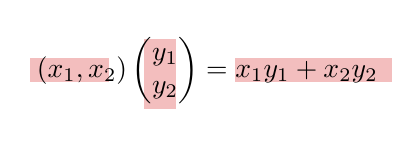
\begin{tikzpicture}
    \definecolor{tab_red}{HTML}{d62728}
    \definecolor{tab_blue}{HTML}{1f77b4}
    \definecolor{tab_green}{HTML}{2ca02c}
    %\draw[help lines] (0,0) grid (8,5);
    \path[fill=tab_red!30] (1.25,0.85) rectangle (2.25,1.15);
    \path[fill=tab_red!30] (2.70,0.50) rectangle (3.10,1.40);
    \path[fill=tab_red!30] (3.85,0.85) rectangle (5.85,1.15);
    
    \node (matrix) at (3.5,1) {
        $\left(x_1, x_2\right)\begin{pmatrix}
            y_1 \cr y_2
        \end{pmatrix} = x_1y_1+x_2y_2$
    };
\end{tikzpicture}
\end{document}